% Things to be done before giving away for print
% - spell check
% - let others proof-read

\documentclass[a4paper,twoside,openright]{report}

%% packages
%%%%%%%%%%%
\usepackage[utf8x]{inputenc}
\usepackage[USenglish]{babel}
\usepackage{amsbsy,amscd,amsfonts,amssymb,amstext,amsmath,amsthm,latexsym}
% Package mathpartir is currently not available in nixpkgs
\usepackage{mathpartir}
\usepackage{stmaryrd}
\usepackage{dot2texi}
\usepackage{url}
\usepackage{hyperref}
\usepackage[xindy]{glossaries}
\usepackage[nottoc]{tocbibind}
\usepackage{pdfpages}

\usepackage{syntax} % for bnf grammar
\usepackage{bussproofs} % for type rules
\usepackage{todonotes}

\usepackage{float} % for figures
\floatstyle{boxed} 
\restylefloat{figure}

\usepackage{listings}
\usepackage{xcolor}
\usepackage{tikz}
\usetikzlibrary{positioning,chains,shapes.arrows,shapes.geometric,fit,calc,arrows,decorations.pathmorphing}

%\usepackage{subfig}
\usepackage{caption}
\usepackage{subcaption}
\usepackage{adjustbox}
\usepackage{cleveref}

%% options
%%%%%%%%%%
% Currently no such things seem to be needed.
% \newtheorem{definition}{Definition}
% \newtheorem{example}{Example}
% \newtheorem{lemma}{Lemma}
% \newtheorem{theorem}{Theorem}
% \newtheorem{claim}{Claim}
% \numberwithin{definition}{chapter}
\bibliographystyle{alphaurl}
\makeglossaries

% some error?
%% macros
%%%%%%%%%
\newcommand{\loremipsum}{\todo[inline]{Lorem Ipsum}}
%\newcommand{\nat}[1]{\ensuremath{\lceil\text{#1}\rceil}}
\newcommand{\gprod}[1]{\ensuremath{\langle\text{#1}\rangle}}
\newcommand{\TNum}{\ensuremath{\mathcal{N}}}
\newcommand{\TBool}{\ensuremath{\mathcal{B}}}
\newcommand{\TInt}{\ensuremath{\mathcal{N}}}

\theoremstyle{definition}
\newtheorem{example}{Example}[chapter]
\newtheorem{definition}[example]{Definition}
%\newtheorem{definition}{Definition}[chapter]

% DCC
% DCC constraints
\newcommand{\pathEq}[2]{\ensuremath{#1 \equiv #2}}
\newcommand{\instanceOf}[2]{\ensuremath{#1 :: #2}}
\newcommand{\instOf}[2]{\instanceOf{#1}{#2}}
\newcommand{\instantiatedBy}[2]{\ensuremath{#1.\textbf{cls} \equiv #2}}
\newcommand{\instBy}[2]{\instantiatedBy{#1}{#2}}
\newcommand{\entails}[2]{\ensuremath{#1 \vdash #2}}
\newcommand*{\ldblbrace}{\{\mskip-6.9mu\{} % left double brace
\newcommand*{\rdblbrace}{\}\mskip-6.9mu\}} % right double brace
\newcommand{\sub}[2]{\ensuremath{\ldblbrace #1 \mapsto #2 \rdblbrace}}

% DCC declarations
\newcommand{\constructorDeclaration}[3]{\ensuremath{#1(#2.\ #3)}}
\newcommand{\constr}[3]{\constructorDeclaration{#1}{#2}{#3}}
\newcommand{\programEntailment}[3]{\ensuremath{ \forall #1.\ #2 \Rightarrow #3}}
\newcommand{\progEnt}[3]{\programEntailment{#1}{#2}{#3}}
\newcommand{\abstractMethodDeclaration}[4]{\ensuremath{#1(#2.\ #3): #4}}
\newcommand{\mDecl}[4]{\abstractMethodDeclaration{#1}{#2}{#3}{#4}}
\newcommand{\methodImplementation}[5]{\ensuremath{#1(#2.\ #3): #4 := #5}}
\newcommand{\mImpl}[5]{\methodImplementation{#1}{#2}{#3}{#4}{#5}}

% DCC expressions
\newcommand{\newInstance}[3]{\ensuremath{\textbf{new } #1(#2 \equiv #3)}}
\newcommand{\newInst}[3]{\newInstance{#1}{#2}{#3}}

% DCC misc
\newcommand{\obj}[3]{\ensuremath{\langle #1; #2 \equiv #3 \rangle}}
\newcommand*{\stdobj}{\ensuremath{\obj{C}{\overline{f}}{\overline{x}}}}
\newcommand{\heap}[2]{\ensuremath{#1 \mapsto #2}}
\newcommand*{\stdheap}{\ensuremath{\heap{\overline{x}}{\overline{o}}}}
\newcommand{\pair}[2]{\ensuremath{\langle #1;#2 \rangle}}
\newcommand{\eval}[4]{\ensuremath{\pair{#1}{#2} \rightarrow \pair{#3}{#4}}}
\newcommand{\typeass}[3]{\ensuremath{#1 \vdash #2 : #3}}
\newcommand{\wf}[1]{\ensuremath{\text{wf }#1}}
\newcommand{\FV}[1]{\ensuremath{FV(#1)}}
\newcommand{\FVeq}[2]{\ensuremath{\FV{#1} = \{#2\}}}

%% misc
%%%%%%%%%
\DeclareMathOperator{\pto}{\rightharpoonup}     % partial function arrow
\DeclareMathOperator{\powerset}{\mathcal{P}}    % powerset
\DeclareMathOperator{\proj}{\upharpoonright}    % projection
\DeclareMathOperator{\fst}{\pi_1}               % A x B → A
\DeclareMathOperator{\snd}{\pi_2}               % A x B → B
\newcommand{\ovl}[1]{\ensuremath{\overline{#1}}}

%%% Local Variables: 
%%% mode: latex
%%% TeX-master: "../thesis"
%%% End: 


\usetikzlibrary{positioning,chains,fit,calc,arrows,decorations.pathmorphing}
\usetikzlibrary{shapes.arrows,shapes.geometric,shapes.symbols}


%%%%%%%
%% tikz stuff
%%%%%%%


\tikzstyle{invisible} = []

\tikzstyle{model}
  = [ shape=rectangle
    , draw
    ]
\tikzstyle{transformation}
  = [ model
    , shape=single arrow
    , draw
    ]

\tikzstyle{meta} = [ double ]
\tikzstyle{generated} = [ dashed ]

\tikzstyle{mopdependency}
  = [ -stealth'
    , semithick
    ]
\tikzstyle{instance}
  = [ mopdependency
    , -open triangle 60
    ]

% Draws the outline of a bend arrow around a rectangle.
% 1. Parameter: name of the rectangle that contains the text
% 2. Parameter: head extend (use 0.25cm to fit with default tikz style)
% 3. Parameter: arc radius (again, 0.25cm seems to work well)
%
% This produces a path, so use it as follows:
%
% \draw[options here] \bendArrow{name of rectangle}{.25cm}{.25cm};
\newcommand{\bendArrow}[3]{
  let \p{content size} = ($(#1.north east) - (#1.south west)$) in
  let \n{tip length 1} = {veclen(0.5 * \y{content size}, 0.5 * \y{content size})} in
  let \n{tip length 2} = {veclen(#2,#2)} in

  (#1.north east)
  -- ++ (315 : \n{tip length 1})
  -- ++ (225 : \n{tip length 1} + \n{tip length 2})
  -- ++ (0, #2)
  -- (#1.south west)
  arc (270 : 180 : \y{content size} + #3)
  -- ++ (\y{content size}, 0)
  arc (180 : 270 : #3)
  (#1.north east)
  -- ++ (135 : \n{tip length 2})
  -- ++ (0, -#2)
  -- (#1.north west)}


%%%%%%%%%%%%%%%%%
%% diagram styles
%%%%%%%%%%%%%%%%%

\tikzstyle{document}
  = [ shape=rectangle
    , draw
    , minimum height=1.5em
    , text width=5em
    , text centered
    ]

\tikzstyle{component}
  = [ font=\scriptsize\it
    ]

\tikzstyle{code}
  = [ shape=rectangle
    , draw
    ]

\tikzstyle{process}
  = [ shape=single arrow
    , single arrow head extend=.75em
    , single arrow head indent=.25em
    , minimum width=3em
    , draw
    ]

\tikzstyle{point}
  = [ coordinate
    , minimum width=1em
    ]

\tikzstyle{flow diagram}
  = [ start chain
    , node distance=1em
    , every node/.style={on chain}
    ]

\tikzstyle{ast}
  = [ node distance=1em and 0.38em
    , every node/.style=ast node
    ]

\tikzstyle{ast node}
  = [ shape=circle
    , minimum size=0.5em
    , inner sep=0
    , fill
    ]

\tikzstyle{dependency}
  = [ dashed
    , -stealth'
    ]

\tikzstyle{red}
  = [ shape=rectangle
    , color=red
    ]

\tikzstyle{blue}
  = [ shape=circle
    , color=blue
    ]

\tikzstyle{green}
  = [ shape=diamond
    , color=green!80!black
    , minimum size=0.7em
    ]

\tikzstyle{note}
  = [ font=\scriptsize\it
    ]
    
\tikzstyle{zoomed arrow}
  = [ solid
    , decorate
    , decoration=snake
    , -stealth'
    ]

\tikzstyle{zoom}
  = [ dashed
    ]

\tikzstyle{uml class}
  = [ shape=rectangle
    , draw
    , font=\sf
    ]

\tikzstyle{uml package}
  = [ uml class
    , inner sep=1em
    ]

\tikzstyle{uml dependency}
  = [ dependency, 
    , dashed
%    , thick
    ]


\newcommand{\bluenode}{\tikz \node [ast node, blue, color=blue, text width=] {};}
\newcommand{\rednode}{\tikz \node [ast node, red, color=red, text width=] {};}
\newcommand{\greennode}{\tikz \node [ast node, green, color=green!80!black, text width=] {};}


\tikzstyle{double arrow}
  = [ shape=double arrow
    , double arrow head extend=.75em
    , double arrow head indent=.25em
    , minimum width=3em
    , draw
    , font=\sf
    ]

%% name graphs

\newdimen\nodedistance
\nodedistance=4em

\tikzstyle{name graph}
  = [ node distance=\nodedistance
    , every node/.style={namenode}
    , every path/.style={ref}
    ]


\tikzstyle{namenode}
  = [ circle
    , thick
    , anchor=center
    , draw
    , minimum size=2em
    , inner sep=2pt
    ]

\tikzstyle{synthesized}
  = [ namenode
    , fill=gray!45
    ]

\tikzstyle{ref}
  = [ -stealth'
    , semithick
    , draw
    ]

\tikzstyle{badref}
  = [ ref
    , dashed
    ]

%% expression trees

\newdimen\nodedistance
\nodedistance=4em

\tikzstyle{exp tree}
  = [ node distance=\nodedistance
    , every node/.style={exp node}
    , every path/.style={link}
    , execute at begin node={\strut}
    ]

\tikzstyle{exp node}
  = [ anchor=center
    ]
\tikzstyle{link}
  = [ semithick
    , draw
    ]

\tikzstyle{ctx node}
  = [ node distance = -.3em,
    ]
\tikzstyle{ctx edge}
  = [ color = red
    , -stealth'
    ]

\tikzstyle{type node}
  = [ node distance = -.5em,
    ]
\tikzstyle{type edge}
  = [ color = blue
    , -stealth'
    ]

%%%%%%%%%%%%%%%%%%%%%%%%%%%
% Pretty printing with tikz
%
% configuration

%%%%%%
%% TikZ and lstlistings
%%%%%%


% remembers a position on the page as a tikz coordinate
\newcommand{\coord}[1]{\tikz[remember picture] \coordinate (#1);}

% translation from baseline to upper border of box
\newcommand{\distanceTop}{7.15pt}

% translation from baseline to lower border of box
\newcommand{\distanceBottom}{-2.55pt}

% translation from baseline to left border of box
\newcommand{\distanceLeft}{-0.5pt}

% translation from baseline to right border of box
\newcommand{\distanceRight}{0.5pt}


% draws a rectangle around 2 points on the page
%
% optional parameter: TikZ style for the line
% 1. mandatory parameter: upper left corner, at text baseline height
% 2. mandatory parameter: lower right corner, at text baseline height
% 3. mandatory parameter: extra margin in all directions
\newcommand{\drawrect}[4][]{\begin{tikzpicture}[remember picture, overlay]
\draw[layout box, #1]
  ($(#2) +(\distanceLeft, \distanceTop) + (-#4, #4)$) rectangle
  ($(#3) + (\distanceRight, \distanceBottom) + (#4, -#4)$);
\end{tikzpicture}}

% draws a rectangle around 2 points on the page
%
% optional parameter: TikZ style for the line
% 1. mandatory parameter: left-hand-side of the first line, at text baseline height
% 2. mandatory parameter: a point on the left side of the rectangle
% 3. mandatory parameter: lower right corner, at text baseline height
% 4. mandatory parameter: extra margin in all directions
\newcommand{\drawbox}[5][]{\begin{tikzpicture}[remember picture, overlay]
\draw[layout box, #1]
  ($(#2) + (\distanceLeft, \distanceTop) + (-#5, #5)$) --
  ($(#4 |- #2) + (\distanceRight, \distanceTop) + (#5, #5)$) --
  ($(#4) + (\distanceRight, \distanceBottom) + (#5, -#5)$) --
  ($(#3 |- #4) + (\distanceLeft, \distanceBottom) + (-#5, -#5)$) --
  ($(#3 |- #2) + (\distanceLeft, \distanceBottom) + (-#5, -#5)$) --
  ($(#2) + (\distanceLeft, \distanceBottom) + (-#5, -#5)$) --
  cycle;
\end{tikzpicture}}

% draws a small \ppBox with three rows around the current point
% #1 = first.col
% #2 = left.col
% #3 = right.col
% #4 = last.col
\newcommand{\drawMiniBox}[4]{
  +(#2 * .2em, 0) --
  +(#2 * .2em, 1ex) --
  +(#1 * .2em, 1ex) --
  +(#1 * .2em, 1.5ex) --
  +(#3 * .2em, 1.5ex) --
  +(#3 * .2em, .5ex) --
  +(#4 * .2em, .5ex) --
  +(#4 * .2em, 0) --
  cycle
}

% A small box (for use inside text)
% optional argument = path options
% #1 = first.col
% #2 = left.col
% #3 = right.col
% #4 = last.col
\newcommand{\minibox}[5][]{%
  \begin{tikzpicture}[baseline=0pt]
  \path [mini layout box, #1]
    (0, 0) \drawMiniBox{#2}{#3}{#4}{#5};
  \end{tikzpicture}}

\newcommand{\miniboxA}{\minibox{-1}{0}{3}{3}}
\newcommand{\miniboxB}{\minibox{0}{0}{3}{3}}
\newcommand{\miniboxC}{\minibox{1}{0}{3}{3}}

% A small rectangle (for use inside text)
\newcommand{\minirect}{\hbox to 9pt{\drawrect[thin,scale=0.3,black]{0pt, 15pt}{26pt, -5pt}{0pt}}}


\tikzstyle{layout box}
  = [ blue
    % , semitransparent
    , semithick
    , draw
    ]

\tikzstyle{mini layout box}
  = [ black
    , very thin
    , draw
    ]

\tikzstyle{annotation}
  = [ font=\small\it
    ]

\tikzstyle{code annotation}
  = [ font=\small\it
    ]


% the font used for pretty printing
\newcommand{\selectCodeFont}{\sf\small}

% the font used for highlighting keywords
\newcommand{\selectKeywordFont}{\bfseries}

% the font used for highlighting string literals
\newcommand{\selectStringLitFont}{\tt}

% the font used for highlighting identifiers
\newcommand{\selectIdentifierFont}{\relax}

% the font used for highlighting operators
\newcommand{\selectOperatorFont}{\tt}

% the text height of token nodes
\newcommand{\tokenHeight}{2ex}

% the text depth of token nodes
\newcommand{\tokenDepth}{.5ex}

%%%%%%%%%%%%%%%%%%%%%%%%%%%
% Pretty printing with tikz
%
% tikz layer

% style for paths or scopes that do pretty printing
\tikzstyle{pretty print}
  = [ start chain=going base right
    , text height=\tokenHeight
    , text depth=\tokenDepth
    , inner sep=0
    , node distance=0em
    ]

% helper style for nodes that start a new line
% (automatically applied by style 'new line' below)
\tikzstyle{new line/helper}
  = [ on chain
    , anchor=north west,
      at={($(#1.west |- \tikzchainprevious.base) + (0, -1.1\baselineskip)$)}
    ]

\tikzstyle{new line tight/helper}
  = [ on chain
    , anchor=north west,
      at={($(#1.west |- \tikzchainprevious.base) + (0, -0.9\baselineskip)$)}
    ]


% style for nodes that start a new line
\tikzstyle{new line}[\tikzchainprevious]
  = [ on chain=placed {new line/helper=#1}
    ]

% style for nodes that start a new line
\tikzstyle{new line tight}[\tikzchainprevious]
  = [ on chain=placed {new line tight/helper=#1}
    ]

% helper style for nodes that tab forward to a labeled position
% (automatically applied by style 'tab forward' below)
\tikzstyle{tab forward/helper}
  = [ on chain
    , anchor=north west,
      at={(#1 |- \tikzchainprevious.base)}
    ]

% style for nodes that tab forward to a labeled position
\tikzstyle{tab forward}
  = [ on chain=placed {tab forward/helper=#1}
    ]

% style for nodes that indent
\tikzstyle{indent}[1em]
  = [ on chain=placed {base right=#1 of \tikzchainprevious}
    ]

% style for nodes that contain an identifier token
\tikzstyle{identifier}
  = [ on chain
    , font=\selectIdentifierFont
    ]

% style for nodes that contain an operator token
\tikzstyle{operator}
  = [ on chain
    , font=\selectOperatorFont
    ]

% style for nodes that contain a keyword token
\tikzstyle{keyword}
  = [ on chain
    , font=\selectKeywordFont
    , text=keyword
    ]

% style for nodes that contain a string literal
\tikzstyle{stringlit}
  = [ on chain
    , font=\selectStringLitFont
    , text=blue
    ]

%%%%%%%%%%%%%%%%%%%%%%%%%%%
% Pretty printing with tikz
%
% \ppBox layer

\newcommand{\Empty}{}
\newcommand{\ignore}[1]{\relax}

\makeatletter
\newcommand{\ppBox}[2][]{{
  % insert keyword token
  \newcommand{\KW}[1]{
    \node[keyword] {##1};
    \HandleToken{\tikzchaincurrent}}

  % insert identifier token
  \newcommand{\ID}[1]{
    \node[identifier] {##1};
    \HandleToken{\tikzchaincurrent}}

  % insert operator token
  \newcommand{\OP}[1]{
    \node[operator] {##1};
    \HandleToken{\tikzchaincurrent}}

  % insert whitespace token
  \newcommand{\SP}{
    \node[on chain] { };
    \HandleInsensitiveToken{\tikzchaincurrent}}

  % label a position (with a tikz node name)
  \newcommand{\LB}[1]{
    \coordinate[on chain] (##1);}

  % tab forward to a labeled position
  \newcommand{\TB}[1]{
    \coordinate[tab forward=##1];
  }

  % insert a string literal
  \newcommand{\STR}[1]{
    \node[stringlit] {##1};
    \HandleToken{\tikzchaincurrent}}

  % insert a line break
  \renewcommand{\\}{
    \coordinate[new line=\NewlineNode];
    \let\HandleToken=\HandleTokenSubsequentLine}

  \newcommand{\newlineTight}{
    \coordinate[new line tight=\NewlineNode];
    \let\HandleToken=\HandleTokenSubsequentLine}

  % the name of the first token
  \let\FirstToken=\Empty
  \newcommand{\AdjustFirst}[1]{
    \ifx\FirstToken\Empty
    \edef\FirstToken{##1}
    \fi
  }

  % the name of the last token
  \let\LastToken=\Empty
  \newcommand{\AdjustLast}[1]{
    \edef\LastToken{##1}
  }

  % the name of the left-most token
  % (except for tokens in the first line)
  \let\LeftToken=\Empty
  \newcommand{\AdjustLeft}[1]{
    \ifx\LeftToken\Empty
      \edef\LeftToken{##1}
    \else
      \pgf@process{\pgfpointanchor{##1}{west}}
      \setlength{\pgf@xa}{\pgf@x}
      \pgf@process{\pgfpointanchor{\LeftToken}{west}}
      \setlength{\pgf@xb}{\pgf@x}
      \ifdim\pgf@xa<\pgf@xb
        \edef\LeftToken{##1}
      \fi
    \fi
  }

  % the name of the rightmost token
  \let\RightToken=\Empty
  \newcommand{\AdjustRight}[1]{
    \ifx\RightToken\Empty
      \edef\RightToken{##1}
    \else
      \pgf@process{\pgfpointanchor{##1}{east}}
      \setlength{\pgf@xa}{\pgf@x}
      \pgf@process{\pgfpointanchor{\RightToken}{east}}
      \setlength{\pgf@xb}{\pgf@x}
      \ifdim\pgf@xa>\pgf@xb
        \edef\RightToken{##1}
      \fi
    \fi
  }

  % this is called for all layout-sensitive tokens in the first
  % line of a pretty printing group
  \newcommand{\HandleTokenFirstLine}[1]{
    \AdjustFirst{##1}
    \AdjustRight{##1}
    \AdjustLast{##1}
  }

  % this is called for all layout-sensitive tokens in subsequent
  % lines of a pretty printing group
  \newcommand{\HandleTokenSubsequentLine}[1]{
    \AdjustLeft{##1}
    \AdjustRight{##1}
    \AdjustLast{##1}}

  % this is called for layout-insensitive tokens in a pretty
  % printing group (such as whitespace, comments, and code that
  % uses explicit layout)
  \newcommand{\HandleInsensitiveToken}[1]{
  }

  % current token handler. will be set to one of:
  %  \HandleTokenFirstLine
  %  \HandleTokenSubsequentLine
  %  \HandleInsensitiveToken
  \newcommand{\HandleToken}[1]{}

  \newcommand{\ppSubBox}[2][]{
    \coordinate[on chain];
    {
      \let\NewlineNode\tikzchaincurrent

      % reset the token registers
      \let\FirstToken=\Empty
      \let\LastToken=\Empty
      \let\LeftToken=\Empty
      \let\RightToken=\Empty

      % start in first line
      \let\HandleToken=\HandleTokenFirstLine

      % typeset content
      ##2

      % draw boundary
      \ifx\LeftToken\Empty
        \path [##1]
          (\FirstToken.north west) rectangle
          (\LastToken.south east);
      \else
        \path [##1]
          (\RightToken.east |- \FirstToken.north) --
          (\FirstToken.north west) --
          (\FirstToken.south west) --
          (\LeftToken.west |- \FirstToken.south) --
          (\LeftToken.west |- \LastToken.south) --
          (\LastToken.south east) --
          (\LastToken.north east) --
          (\RightToken.east |- \LastToken.north) --
          cycle;
      \fi

      % remember the token registers outside the group
      \global\let\InnerFirstToken=\FirstToken
      \global\let\InnerLastToken=\LastToken
      \global\let\InnerLeftToken=\LeftToken
      \global\let\InnerRightToken=\RightToken

      % remember the state outside the group
      \global\let\InnerHandleToken=\HandleToken
    }
    % handle the significant inner tokens
    % and significant inner linebreaks
    \HandleToken{\InnerFirstToken}
    \ifx\HandleToken\HandleTokenFirstLine
    \let\HandleToken=\InnerHandleToken
    \fi
    \ifx\InnerLeftToken\Empty
    \else
    \HandleToken{\InnerLeftToken}
    \fi
    \HandleToken{\InnerRightToken}
    \HandleToken{\InnerLastToken}
  }

  % indent a ppBox
  \newcommand{\IN}[1]{\coordinate[indent]; ##1}
  \newcommand{\DE}[1]{\coordinate[indent=-1em]; ##1}

  \let\ppBox=\ppSubBox
  \ppBox[#1]{#2}}}
\makeatother




%%% Local Variables: 
%%% mode: latex
%%% TeX-master: "../thesis"
%%% End: 

%\input{include/glossary}

\begin{document}

% Title page
%%%%%%%%%%%%
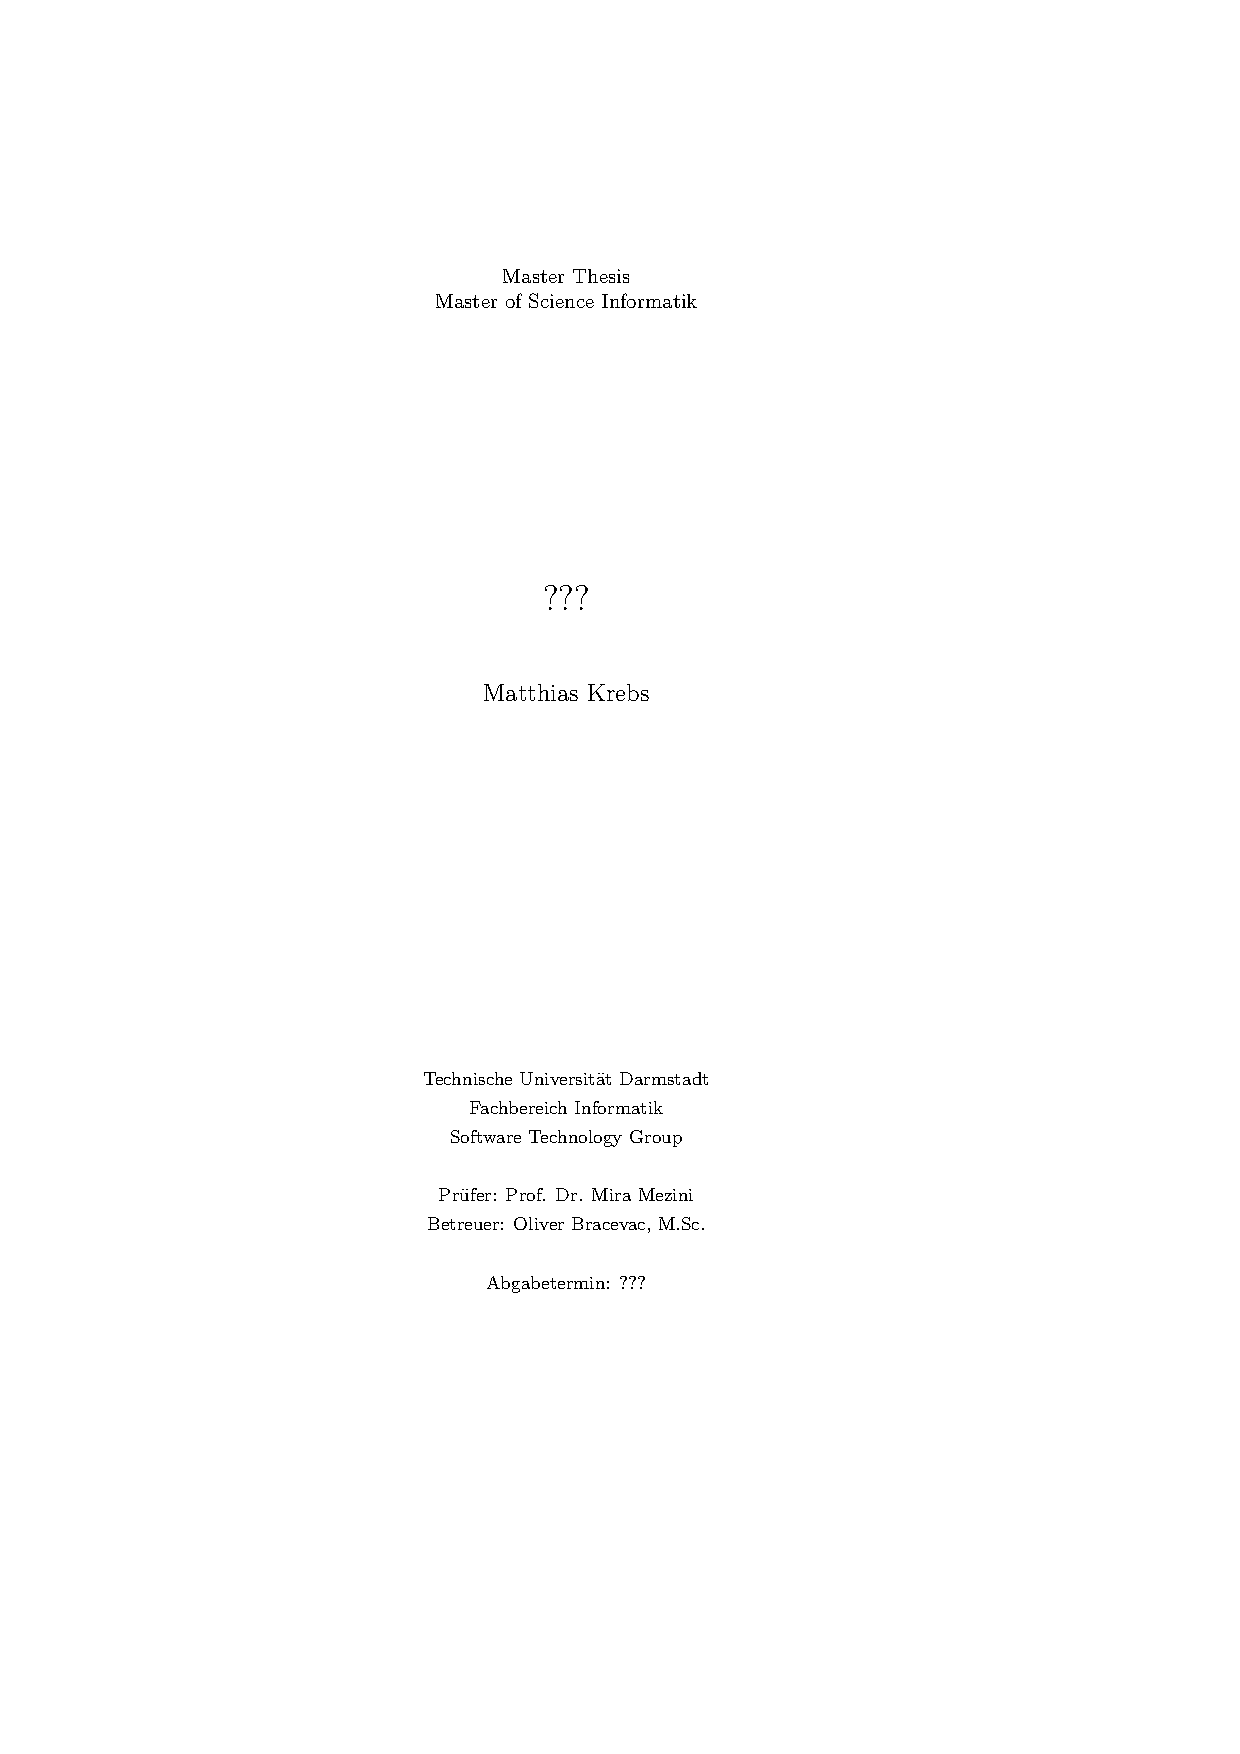
\includepdf{titlepage.pdf}

\clearpage
\thispagestyle{empty}
\mbox{}

% Erklärung
%%%%%%%%%%%
\newpage
\thispagestyle{empty}
\section*{Erklärung}
Hiermit versichere ich, Matthias Krebs, die vorliegende Master-Thesis
gemäß § 22 Abs. 7 APB der TU Darmstadt ohne Hilfe Dritter und nur mit
den angegebenen Quellen und Hilfsmitteln angefertigt zu haben.
Alle Stellen, die Quellen entnommen wurden, sind als solche kenntlich
gemacht worden. Diese Arbeit hat in gleicher oder ähnlicher Form noch
keiner Prüfungsbehörde vorgelegen.
\newline\newline
Mir ist bekannt, dass im Falle eines Plagiats (§38 Abs.2 APB) ein
Täuschungsversuch vorliegt, der dazu führt, dass die Arbeit mit 5,0
bewertet und damit ein Prüfungsversuch verbraucht wird.
Abschlussarbeiten dürfen nur einmal wiederholt werden.
\newline\newline
Bei der abgegebenen Thesis stimmen die schriftliche und die zur
Archivierung eingereichte elektronische Fassung gemäß § 23 Abs. 7 APB überein.

\vskip 2cm
\parbox{4cm}{\centering\hrule
\strut \centering\footnotesize Ort, Datum} \hfill\parbox{4cm}{\hrule
\strut \centering\footnotesize (Matthias Krebs)}
\newpage

%%% Local Variables:
%%% mode: latex
%%% TeX-master: "../thesis"
%%% End:


% Abstract
%%%%%%%%%%
\begin{abstract}
- dependent classes
  - support:
  - dynamic dispatch (polymorphic methods)
  - inheritance
  - on the level of groups of related classes
- DCC calculus extends the semantics of dependent classes with abstract classes and methods
  and expresses inheritance through a constraint system
- we implement the DCC calculus
- and solve the constraint system by using SMT solving
- we propose "context enrichment" as a process
  of transferring compile time information to the runtime of a program
  to increase the performance of the constraint system solving

%%% Local Variables: 
%%% mode: latex
%%% TeX-master: "../thesis"
%%% End: 

\end{abstract}

% Table of contents
%%%%%%%%%%%%%%%%%%%
\tableofcontents

% Content
%%%%%%%%%
\chapter{Introduction}
\section{Motivation}
Dynamic dispatch is the process to determine
the implementation of a polymorphic method
to call at runtime.
In contrast to static dispatch,
which determines this during compile time.
%
Safety describes the ability of a language
to prevent errors.
%
In object oriented programming
related classes can be grouped together,
but inheritance between those groups can not be expressed.

Dependent Classes~\cite{dc} combine dynamic dispatch à la Smalltalk~\cite{smalltalk}
with safety à la Scala~\cite{scala},
as well as supporting inheritance between groups of related classes.
The support for abstract methods is yet to be fully explored.
The $DC_C$ calculus by Vaidas Gasiūnas~\cite{vaidas:thesis}
captures the semantics of Dependent Classes
and extends it with the support for abstract classes and methods.
Subtyping in the $DC_C$ calculus is expressed as constraint entailment.

The goal of this thesis is to implement the $DC_C$ calculus
and to explore the usage of SMT to solve the constraint system of the calculus.

%- dynamic dispatch
%  - selecting which implemenetation of a polymorphic method to call at runtime
%  - in contrast to static dispatch which does this at compile time
%- (type) safety
%  - describes the ability to discourage/prevent errors (during compile time? → not really, dynamic typing)
%- dependent calsses
%  - combine dynamic dispatch and safety
%  - not yet/still a problem: abstract methods
%  - DCC calculus by vaidas: dependent classes with abstract methods
%  - subtyping can be described/expressed as constraint entailment
%  - not much explored in an object oriented setting
%  - use SMT solver to explore it

\section{Contributions}
The main contributions of the thesis are:
\begin{itemize}
  \item An implementation of the $DC_C$ calculus
        using SMT solving to resolve the constraint system.
  \item A first-order model of the $DC_C$ constraint system,
        which translates the rules of a sequent calculus
        to universal quantified formulae.
  \item Optimizations to the rules of the first-order model,
        such that a SMT solver can make better use of them.
  \item An implementation of the $DC_C$ relation for
        type assignments to expressions.
  \item A way to use type information of an expression
        in the interpretation of that expression
        to reduce the time to solve the constraint system.
\end{itemize}

\section{Structure}
\Cref{chp:pre} presents preliminaries.
We introduce Satisfiability Modulo Theories,
Dependent Classes and the $DC_C$ calculus.\\
\\
\Cref{chp:impl} gives an implementation of the $DC_C$ calculus.
We implement
the constraint system in \Cref{sec:constraintsystem},
the operational semantics in \Cref{sec:interp} and
the type relation in \Cref{sec:types}.\\
\\
\Cref{chp:eval} gives applications of the interpreter
to a $DC_C$ program and
evaluates which expressions the interpreter can successfully reduce.\\
\\
\Cref{chp:learning} presents an approach
to use information gained from compile time (type checker)
during runtime (interpreter).\\
\\
Related work is discussed in \Cref{chp:related}
and we conclude the thesis in \Cref{chp:discuss}.

%%% Local Variables: 
%%% mode: latex
%%% TeX-master: "../thesis"
%%% End: 

\clearpage
\chapter{Preliminaries}
\label{chp:pre}
\section{Satisfiability modulo theories}
\label{sec:smt}
Many problems like formal verification of hard- and software can be reduced
to checking the satisfiability of a formula in some logic.
Some of these problems can be easily described as a satisfiability problem
in propositional logic and solved using a propositional SAT solver.
Other problems can be described more naturally in other classical logics like first-order logic.
These logics support more expressive language features including
non-boolean variables, function and predicate-symbols and quantifiers.

The defining problem of Satisfiability modulo theories (SMT)
is checking if a logical formula is satisfiable in the context of some background theory.
Checking validity can be achieved using SMT if the formula is closed under logical negation,
since a formula is valid in a theory if it's negation is not satisfiable in the theory.

There is a trade-off between the expressiveness of a logic and
the ability to automatically check satisfiability of formulae.
A practical compromise is the usage of fragments of first-order logic,
where the used fragment is restricted syntactically or semantically. % TODO: add examples for restrictions, see notes
Such restrictions achieve the decidability of the satisfiability problem and
allow the development of procedures that exploit properties of the fragment for efficiency.
A SMT solver is any software implementing a procedure for determining satisfiability modulo a given theory.
SMT solvers can be distinguished based on the underlying logic (first-order, modal, temporal, ...),
the background theory, the accepted input formulas and the interface provided by the solver.\cite{smt,smtlib}
Z3 is a SMT solver from Microsoft Research\cite{z3}, which is used in this thesis.
%- SMT problem
%    - is logical formular satisfiable given a logical theory
%- propositional SAT solver
%- some problems described more naturally in classical logics
%    - such as fo or higher order logics
%    - with more expressive features/languages
%    - including non-Boolean variables, function and predicate-symbols (positive arity), quantifiers
%- trade-off between expressivenes of logic and ability of automatically checking satisfiability of formulae
%- practical compromise: use fragments of first-order logic
%    - fragment is restricted
%        - syntactically and/or
%        - constraining the interpretation of certain function and predicate symbols
%        - makes the satisfiability problem decidable
%        - allows development of procedures that exploit properties of the fragment for efficiency

\subsection{SMT-Lib}
SMT-Lib is a international initiative with the goal to easing
research and development in SMT.
SMT-Lib's main motivation is the availability of common standards in SMT
with the focused on
\begin{itemize}
    \item providing a standard description of background theories
    \item developing a common in- and output language for SMT solvers
    \item establishing a library of benchmarks for SMT solvers
\end{itemize}
to advance the state of the art in the field.
The SMT-Lib Standard: Version 2.6\cite{smtlib} defines a language for
writing terms and formulas in sorted first-order logic,
specifying background theories,
specifying logics,
as well as a command language for interacting with SMT solvers.
The SMT-Lib format is accepted by the majority of current SMT solvers.
%- SMT-Lib international initiative aimed at facilitating research and developmentin SMT
%- focused on
%    - provide standard rigorous descriptions of background theories used in SMT
%    - develop + promote common in/output language for SMT solvers
%    - establish library of benchmarks for SMT solvers
%- main motivation for SMT-Lib: availability of common standards
%    and of library of benchmarks facilitate evulution and comparison for SMT systems
%- advance the state of the art in the field
%- SMT-Lib format is accepted by majority of current SMT solvers
%- SMT-Lib Standard 2.6 defines
%    - language for writing terms and formulas in sorted fo
%    - language for specifying background theories
%        - standard vocabulary of sort, function and predicate symbols
%    - language for specifying logics
%        - suitably restricted classes of formulas
%    - command language for interacting with SMT solvers
%        - asserting and retracting formulas
%        - querying about satisfiability
%        - examining models or unsat proofs
%        - ...
An example of the SMT-Lib format is shown in figure 2.1. %TODO: figure numbering style?
The example is showing a formula in sorted first-order logic and the SMT-Lib representation of the formula.
The formula is quantifying over two integer lists,
using a let binding to extract the head and the tail from the first list
to construct a identical list out of these bindings and checks for equality to the second list.
The example is purely for demonstrating the syntax of the SMT-Lib format.

\begin{figure}
\begin{align*}
&\forall x: List[Int]. \exists y: List[Int]. \\
&\text{ let } h := head(x), t := tail(x)\\
&\text{ in } insert(h, t) = y
\end{align*}
\begin{center}
(forall ((x (List Int))) (exists ((y (List Int))) \\
(let ((h (head x)) (t (tail x))) \\
(= (insert h t) y))))
\caption{SMT-Lib format example}
\end{center}
\end{figure}

\section{Dependent Classes}
\label{sec:depcls}
Classes tend to be a too isolated unit to achieve modularity.
Desired functionality involves groups of related classes.
Grouping mechanisms exist, like namespaces in C++ and packages in Java,
but these mechanisms do not cover inheritance and polymorphism for expressing variability.
Virtual classes\cite{virtual:classes, vaidas:thesis} provide a solution for inheritance and polymorphism.
They introduce classes as a kind of object members and treat these as virtual methods,
which allows for overriding in subclasses and are late-bound.
Virtual classes are inner classes refinable in the subclasses of the enclosing class.
%- classes not good enough for modularity
%- functionality involves a group of related classes
%- grouping mechanisms (namespaces, packages, ...)
%- does not cover inheritance and polymorphism for expressing variability
%- virtual classes \cite{virtual:classes}
%    - provide solution for inheritance and polymorphism
%    - introduce classes as "object members" and treat them like (virtual) methods
%        - allow overriding in subclasses, late-bound
%    - are inner classes that can be refined in the subclasses of the enclosing class

The downside of Virtual Classes is that they must be nested within other classes.
This requires to cluster classes depending on instances of some class together,
introducing maybe unwanted coupling between these classes.
Introducing a new class depending on the instances of an existing class
requires the modification this class and its subclasses,
limiting extensibility.
This Nesting does also limit the expression of variability:
The interface and the implementation of a virtual class can only depend
on its single enclosing object.

Dependent classes\cite{dc,vaidas:thesis} are generalization of virtual classes.
The structure of a dependent class depends on arbitrarily many objects and
dependency is expressed with class parameters.
Dependent classes can be seen as a combination of virtual classes with multi-dispatch.

The semantics of dependent classes involve non-trivial aspects,
such as method calls and class instantiation expressions,
which rely on dynamic dispatch over multiple parameters and the types of their fields.
As well as the complexity of the type system,
which integrates static dispatch with dependent typing.
%- semantics of dependent classes
%    - invole multiple non-trivial aspects
%    - method calls and class instantiation expressions rely on dynamic dispatch over multiple parameters
%        and the types of fields
%    - most of the complexity in type system
%        - integrates static dispatch with dependent typing

The $vc^n$ calculus captures the core semantics of dependent classes,
such as static and dynamic dispatch and dependent typing based on paths.
The calculus ensures that the static dispatch and static normalization of terms in types
define a proper abstraction over dynamic dispatch and evaluation of expressions.
It is defined in an algorithmic style.
This algorithmic style has the advantage of being constructive
and through this outlining a possible implementation.
The algorithmic nature of the calculus comes also with the disadvantage
of being difficult to extend semantics with new expressive power,
such as extending the calculus with support for abstract declarations.
%- vcn calculus
%    - captures core semantics of dependent classes,
%        including static and dynamic dispatch and dependent typing based on paths
%    - calculus defined to ensure static dispatch and static normalization of terms in types
%        defines proper abstraction over dynamic dispatch and evaluation of expressions
%    - defined in an algorithmic style
%        - for ensuring decidability of type system through straightforward proof TODO: add this?
%    - algorithmic style has advantage of being constructive -> outlines a possible implementation
%    - at the same time disadvantage: difficult to extend semantics with new expressive power
%        - difficult to extend calculus with support for abstract declarations

\subsection{$DC_C$ Calculus}
\label{sec:dcc}
The $vc^n$ calculus does not support abstract classes and methods.
The $DC_C$ calculus~\cite{vaidas:thesis} extends $vc^n$ with support for abstract classes and methods
and symmetric method dispatch.
$DC_C$ encodes dependent classes with a constraint system,
which is used in both the static and dynamic semantics.
The main relation of the $DC_C$ calculus is constraint entailment.
%replacing $vc^n$'s relations for type equivalence, subtyping, static and dynamic dispatch.

The runtime structure is heap-based,
with explicit object identities
and relationships between objects based on these identities.
Expressions evaluate to an identifier pointing to an object in the heap.
Heaps preserve object identity and enable shared references to objects.
The heap provides a direct interpretation for equivalent paths,
two paths are equivalent if they point to the same object at runtime.
Heaps can be easily translated to a set of constraints describing its objects and their relations,
which enables the usage of the constraint system for dynamic dispatch and expression typing.
%- DCc extends $vc^n$ with abstract methods and classes and symmetric method dispatch
%- gave up unification of methods and classes
%- runtime structure: heap
%- heap structure preserves object identity, enables shared references
%- heap provides direct interpretation for equivalent paths
%    - paths are equiv if they point to the same object at runtime
%- heaps can be easily translated to a set of constraints describing its objects and their relations
%    - enables using constraint system for dynamic dispatch and expression typing
\\ \\
Here we show the calculus by Vaidas Gasiūnas.
\subsubsection{Syntax}
% begin syntax figure
\begin{figure}[t]
\begin{align*}
\mathit{Program} &::= \ovl{Decl} \\
\mathit{Decl} &::= \constr{C}{x}{\overline{Constr}} % C(x. $\overline{Constr}$)
                 \ |\ \progEnt{x}{\overline{Constr}}{Constr} \\
              &\ \ |\ \mDecl{m}{x}{\overline{Constr}}{Type} % m(x. $\overline{Constr}$): Type
                 \ |\ \mImpl{m}{x}{\overline{Constr}}{Type}{Expr} \\ % m(x. $\overline{Constr}$): Type := Expr
\mathit{Type} &::= \type{x}{\ovl{Constr}} \\
\mathit{Constr} &::= \pathEq{Path}{Path} % Path $\equiv$ Path
                \ |\ \instOf{Path}{C} % Path :: C
                \ |\ \instBy{Path}{C} \\ % Path.\textbf{cls} $\equiv$ C
\mathit{Path} &::= x \ |\ \mathit{Path.f}\\
\mathit{Expr} &::= x
              \ |\ \mathit{Expr.f}
              \ |\ \newInst{C}{\overline{f}}{\overline{Expr}} % \textbf{new} C($\overline{f}$ $\equiv$ $\overline{Expr}$)
              \ |\ m(\mathit{Expr})
\end{align*}
%\hrule
\begin{align*}
MType(m, x, y) &= \{ \langle\overline{a}, \overline{b}\rangle | (m(x. \overline{a}): \type{y}{\ovl{b}}...) \in P \} \\
MImpl(m, x) &= \{\langle\overline{a}, e\rangle | (m(x. \overline{a}): \type{y}{\ovl{b}} := e) \in P \}
\end{align*}

$x, y \in$ variable names\\
$f \in$ field names\\
$C \in$ class names\\
$m \in$ method names
\caption{Syntax}
\label{fig:dcc-syntax}
\end{figure}
% end syntax figure
The syntax of $DC_C$ is given in \Cref{fig:dcc-syntax}.
Types are lists of constraints to be satisfied by their instances.
Types have the form \type{x}{\ovl{a}}, where $x$ is a bound variable
and \ovl{a} is a list of constraints on $x$.
An object belongs to a type if it fulfills its constraints.

Constraints of the form $p \equiv q$ express that two paths $p$ and $q$ are equivalent
and paths are considered to be equivalent if they refer to the same object at runtime.
$p :: C$ specifies that path $p$ refers to an instance of class $C$.
The stronger form $p.\textbf{cls} \equiv C$ denotes that
path $p$ refers to an object instantiated by a constructor of class $C$,
excluding indirect instances of $C$ inferred through inheritance rules.

A Program $P$ consists of a list of declarations $D$.
Possible declarations are constructor declarations,
abstract method declarations, method implementations and constraint entailment rules.

A Path expression can be a variable $x$ or navigation over fields starting from a variable e.g. $x.f$.

Expressions can be variables, field access, object construction and method invocation.
Field assignments are not supported since the calculus is functional.
%
\begin{example}[Natural Numbers]
\label{ex:dcc-naturalnumbers}
\begin{align*}
&\constr{\texttt{Zero}}{x}{\epsilon}\\
&\progEnt{x}{\instOf{x}{\texttt{Zero}}}{\instOf{x}{\texttt{Nat}}}\\
&\constr{\texttt{Succ}}{x}{\instOf{x.p}{\texttt{Nat}}}\\
&\progEnt{x}{\instOf{x}{\texttt{Succ}}, \instOf{x.p}{\texttt{Nat}}}{\instOf{x}{\texttt{Nat}}}\\
&\mDecl{\texttt{prev}}{x}{\instOf{x}{\texttt{Nat}}}{\type{y}{\instOf{y}{\texttt{Nat}}}}\\
&\mImpl{\texttt{prev}}{x}{\instOf{x}{\texttt{Zero}}}{\type{y}{\instOf{y}{\texttt{Nat}}}}{\newInstNoArgs{\texttt{Zero}}}\\
&\mImpl{\texttt{prev}}{x}{\instOf{x}{\texttt{Succ}}, \instOf{x.p}{\texttt{Nat}}}{\type{y}{\instOf{y}{\texttt{Nat}}}}{x.p}
\end{align*}
\end{example}
%
\Cref{ex:dcc-naturalnumbers} shows a program defining natural numbers.
The program has constructors \texttt{Zero} representing zero
and \texttt{Succ} representing the successor of its field $p$.
The inheritance of \texttt{Zero} and \texttt{Succ} to \texttt{Nat}
is expressed through the two constraint entailment rules.
The method \texttt{prev}is abstractely declared to
be a function from \texttt{Nat} to \texttt{Nat}.
It has two implementations,
one for \texttt{Zero} and one for \texttt{Succ}.

\subsubsection{Constraint System}
% begin constraint system figure
\begin{figure}[t]
% C-Ident
\begin{prooftree}
\AxiomC{}
\RightLabel{(C-Ident)}
\UnaryInfC{\entails{a}{a}}
\end{prooftree}
% C-Refl
\begin{prooftree}
\AxiomC{}
\RightLabel{(C-Refl)}
\UnaryInfC{\entails{\epsilon}{\pathEq{p}{p}}}
\end{prooftree}
% C-Class
\begin{prooftree}
\AxiomC{\entails{\overline{a}}{\instantiatedBy{p}{C}}}
\RightLabel{(C-Class)}
\UnaryInfC{\entails{\overline{a}}{\instanceOf{p}{C}}}
\end{prooftree}
% C-Cut
\begin{prooftree}
\AxiomC{\entails{\overline{a}}{c}}
\AxiomC{\entails{\overline{a'}, c}{b}}
\RightLabel{(C-Cut)}
\BinaryInfC{\entails{\overline{a},\overline{a'}}{b}}
\end{prooftree}
% C-Subst
\begin{prooftree}
\AxiomC{\entails{\overline{a}}{a_{\sub{x}{p}}}}
\AxiomC{\entails{\overline{a}}{\pathEq{p'}{p}}}
\RightLabel{(C-Subst)}
\BinaryInfC{\entails{\overline{a}}{a_{\sub{x}{p'}}}}
\end{prooftree}
% C-Prog
\begin{prooftree}
\AxiomC{$(\progEnt{x}{\overline{a}}{a}) \in P$}
\AxiomC{\entails{\overline{b}}{\overline{a}_{\sub{x}{p}}}}
\RightLabel{(C-Prog)}
\BinaryInfC{\entails{\overline{b}}{a_{\sub{x}{p}}}}
\end{prooftree}
\caption{Constraint Entailment}
\label{fig:dcc-constraint-entailment}
\end{figure}
% end constraint system figure
The constraint system is given in the style of the sequent calculus
and the rules for the constraint system are specified in \Cref{fig:dcc-constraint-entailment}.
The sequent \entails{\ovl{a}}{a} is interpreted as constraint entailment:
constraints \ovl{a} entail constraint $a$.
The constraints on the left-hand side are referred to as the context
and the constraint on the right-hand side as the constraint entailed by the context.
The notion \entails{\ovl{a}}{\ovl{b}} is used differently than in the sequent calculus.
For $DC_C$ it is used as a shortcut for a list of judgments
\entails{\ovl{a}}{b_i} for each $b_i \in \ovl{b}$,
meaning that all $b_i$ are entailed by \ovl{a}.

Rules C-Ident and C-Cut are standard rules of the sequent calculus,
the remainder of the rules are specific to the programming language.
The standard structural rules of the sequent calculus allowing
permutation, weakening and contraction of the context
are implicitly assumed to be specified.

The properties of path equivalence are specified with rules C-Refl and C-Subst.
Rule C-Refl establishes reflexivity of path equivalence.
Rule C-Subst specifies that paths can be substituted with equivalent paths
at any position of any other constraint.
Other typical rules of equivalence as symmetry and transitivity can be
derived from these rules.

Rule C-Class specifies that a direct instance of a class
is an instance of that class, describing that
\instOf{p}{C} is a weaker relationship than \instBy{p}{C}.

With Rule C-Prog it is possible to specify new axioms for the constraint system in programs.
This is used to express inheritance declarations between dependent classes:
the constraint at the right-hand side of the implication must be \instOf{x}{p},
where $x$ is the bound variable of the rule.
The rule is restricted to avoid an undecidable constraint system
and the restrictions are specified by the well-formedness rule WF-RD in \Cref{fig:dcc-wf}.

\subsubsection{Operational Semantics}
The operational semantics is given in \Cref{fig:dcc-opsemantics}.
It is defined as a small-step reduction relation of a heap and an expression.
A heap is a list of mappings from variables to objects.
Each object is specified by a class and a list of the values of its fields,
which are again references in the heap.
For heaps $h$ and variables $x$, $h(x)$ denotes the object of $h$ referenced by $x$.

The function $HC$ takes a heap and gives the constraints satisfied by all variables of the heap.
The function $OC$ converts an object %definition TODO: keep this?
to a list of constraints on a given variable.
A Constraint $a$ is satisfied by a heap $h$, if $\entails{HC(h)}{a}$ holds.

Evaluation in $DC_C$ is a process of moving information from the expression to the heap
and the values of $DC_C$ are references in the heap.
Evaluation must yield a heap and a variable.
During reduction only new objects can be added to the heap,
while existing objects remain unchanged.

The congruence rules RC-Field, RC-New and RC-Call propagate reduction to subexpressions.
The computation rules R-Field, R-New and R-Call can only be applied
when all subexpressions of an expression are reduced to normal forms (variables).

Field access $x.f$ is reducible to the value of $x.f$ in the heap
if the heap constraints include \pathEq{x.f}{y},
where $y$ represents the value retrieved from the heap.
$x$ does not have field $f$ in the heap if the constraint is not included.

Object construction \newInst{C}{\ovl{f}}{\ovl{x}} is reduced
to a fresh variable $x$ representing the new object,
as well as extending the heap with an object $o = \obj{C}{\ovl{f}}{\ovl{x}}$ of class $C$ with
\ovl{x} as the values of the fields of that object.
It is checked that a constructor of class $C$ exists in the program
and that the constraints \ovl{b} specified by the constructor
are satisfied by the new object \entails{HC(h),OC(x,o)}{\ovl{b}}.

A method call $m(x)$ is reduced to the body of the most specific applicable method implementation.
Applicability of the implementations and selection of the most specific one
are determined by constraints.
A method declaration is applicable if its arguments are entailed by the context.
Set $S$ contains the applicable methods.
A method declaration with argument constraints \ovl{a}
is more specific than a method declaration with argument constraints \ovl{a'}
if \entails{\ovl{a'}}{\ovl{a}},
but not the other way around $\neg\entails{\ovl{a}}{\ovl{a'}}$.

\subsubsection{Type Checking}
\label{sec:dcc-types}
% begin Type assignment figure
\begin{figure}
% T-Field
\begin{prooftree}
\AxiomC{\typeass{\ovl{c}}{e}{\type{x}{\ovl{a}}}}
\AxiomC{\entails{\ovl{c},\ovl{a}}{\instOf{x.f}{C}}}
\AxiomC{\entails{\ovl{c}, \ovl{a}, \pathEq{x.f}{y}}{\ovl{b}}}
\AxiomC{$x \not \in \FV{\ovl{b}}$}
\RightLabel{T-Field}
\QuaternaryInfC{\typeass{\overline{c}}{e.f}{\type{y}{\ovl{b}}}}
\end{prooftree}
% T-Var
\begin{prooftree}
\AxiomC{\entails{\ovl{c}}{\instOf{x}{C}}}
\RightLabel{T-Var}
\UnaryInfC{\typeass{\ovl{c}}{x}{\type{y}{\pathEq{y}{x}}}}
\end{prooftree}
% T-Call
\begin{prooftree}
\AxiomC{\entails{\ovl{c}, \ovl{a}}{\ovl{a'}}} % 3
\AxiomC{\typeass{\ovl{c}}{e}{\type{x}{\ovl{a}}}} % 1
\AxiomC{$\pair{\ovl{a'}}{\ovl{b}} \in MType(m, x, y)$} % 2
\noLine
\BinaryInfC{\entails{\ovl{c},\ovl{a},\ovl{b}}{\ovl{b'}}} % 4
\AxiomC{$x \not \in \FV{\ovl{b'}}$} % 5
\RightLabel{T-Call}
\TrinaryInfC{\typeass{\ovl{c}}{m(e)}{\type{y}{\ovl{b'}}}}
\end{prooftree}
% T-New
\begin{prooftree}
\AxiomC{$\forall i.\ \typeass{\ovl{c}}{e_i}{\type{x_i}{\ovl{a_i}}}$} % 1
\noLine
\UnaryInfC{$\ovl{b} = (\instBy{x}{C}), \bigcup_i \ovl{a_i}_{\sub{x_i}{x.f_i}}$} % 3
\AxiomC{$\constr{C}{x}{\ovl{b'}} \in P$} % 2
\noLine
\UnaryInfC{\entails{\ovl{c},\ovl{b}}{\ovl{b'}}} % 4
\RightLabel{T-New}
\BinaryInfC{\typeass{\ovl{c}}{\newInst{C}{\ovl{f}}{\ovl{e}}}{\type{x}{\ovl{b}}}}
\end{prooftree}
% T-Sub
\begin{prooftree}
\AxiomC{\typeass{\ovl{c}}{e}{\type{x}{\ovl{a'}}}}
\AxiomC{\entails{\ovl{c},\ovl{a'}}{\ovl{a}}}
\RightLabel{T-Sub}
\BinaryInfC{\typeass{\ovl{c}}{e}{\type{x}{\ovl{a}}}}
\end{prooftree}
\caption{Type Assignment}
\label{fig:dcc-typeass}
\end{figure}
% end Type assignment figure
Type assignment for expressions is defined in \Cref{fig:dcc-typeass}.
The context of type assignment is a list of constraints providing information
about variables that occur in the expression.
The typing rules ensure that all free variables of the assigned types
appear in the context.
An expression type \type{x}{\ovl{a}} is a collection of constraints \ovl{a}
with a bound variable $x$
that will hold for all possible values of the expression at runtime,
if the runtime environment satisfies the constraints of the context.
The relation does not guarantee unique type assignments,
since it is possible to have different constraints satisfied by an expression.
The rule T-Sub explicitly allows weakening the type of an expression.

The type of a variable $x$ is specified by rule T-Var.
The type of $x$ asserts equivalence of the bound variable $y$ of the type to $x$.
Further it is checked that \instOf{x}{C} can be satisfied by the context for some class $C$.

Rule T-Field specifies type assignment of a field access $e.f$.
The constraints of such a field access are the constraints on $x.f$
entailed by the type of $e$
, where $x$ is the bound variable of the type of $e$.
The elimination of $x$ is done via the usage of
constraints free of $x$ entailed by the type of $e$ and \pathEq{y}{x.f},
where $y$ is used as the bound variable of the type of $e.f$
and \entails{\ovl{c},\ovl{a}}{\instOf{x.f}{C}} is used to check if
field $f$ of $e$ is available at runtime.

Rule T-Call specifies type assignment of method calls $m(e)$.
The type of $e$ is \type{x}{\ovl{a}}.
The rule checks the existence of a declaration of $m$,
whose parameter constrains are \ovl{a'} and return type constraints are \ovl{b}.
It is checked with \entails{\ovl{c},\ovl{a}}{\ovl{a'}} if
the parameter constraints are entailed by the type of $e$.
The type constraints of $m(e)$ are derived from the declared return type of $m$
and the type of the argument $e$.
The argument variable $x$ is eliminated, because it does not appear in the context
and the entailed constraints of the return types and the argument types
free of $x$ are taken.

Rule T-New specifies type assignment of object constructions.
The type \type{x}{\ovl{b}} of an object construction \newInst{C}{\ovl{f}}{\ovl{e}}
consists of a constraint stating that $C$ is the class of the object and the constraints of its fields.
The field constraints are taken from the types of the expressions $e_i$
assigned to the fields $f_i$.
Additionally \entails{\ovl{c},\ovl{b}}{\ovl{b'}} checks
that the new object satisfies the constraints of at least
one constructor \constr{C}{x}{\ovl{b'}} of class $C$.
\\
\\
% begin Type Checking figure
\begin{figure}[t]
% WF-CD
\begin{prooftree}
\AxiomC{\FVeq{\ovl{a}}{x}}
\RightLabel{WF-CD}
\UnaryInfC{\wf{\constr{C}{x}{\ovl{a}}}}
\end{prooftree}
% WF-MS
\begin{prooftree}
\AxiomC{\FVeq{\ovl{a}}{x}}
\AxiomC{\FVeq{\ovl{b}}{x,y}}
\RightLabel{WF-MS}
\BinaryInfC{\wf{(\mDecl{m}{x}{\ovl{a}}{\type{y}{\ovl{b}}})}}
\end{prooftree}
% WF-RD
\begin{prooftree}
\AxiomC{\FVeq{\ovl{a}}{x}}
\AxiomC{$\instOf{x}{C'} \in \ovl{a}$}
\RightLabel{WF-RD}
\BinaryInfC{\wf{(\progEnt{x}{\ovl{a}}{\instOf{x}{C}})}}
\end{prooftree}
% WF-MI
\begin{prooftree}
\AxiomC{\FVeq{\ovl{a}}{x}}
\AxiomC{\FVeq{\ovl{b}}{x,y}}
\AxiomC{\typeass{\ovl{a}}{e}{\type{y}{\ovl{b}}}}
\RightLabel{WF-MI}
\TrinaryInfC{\wf{(\mImpl{m}{x}{\ovl{a}}{\type{y}{\ovl{b}}}{e})}}
\end{prooftree}
% WF-Prog
\begin{prooftree}
\AxiomC{$\forall D \in P.\ \wf{D}$}
\noLine
\UnaryInfC{$\forall m.\ \forall \pair{\ovl{a}}{\ovl{b}}, \pair{\ovl{a'}}{\ovl{b'}} \in MType(m, x, y).\ \ovl{b} = \ovl{b'}$}
\noLine
\UnaryInfC{$\forall m.\ unique(m)$}
\noLine
\UnaryInfC{$\forall m.\ \forall \pair{\ovl{a}}{\ovl{b}} \in MType(m, x, y).\ complete(m, \type{x}{\ovl{a}})$}
\RightLabel{WF-Prog}
\UnaryInfC{\wf{P}}
\end{prooftree}
\caption{Type Checking}
\label{fig:dcc-wf}
\end{figure}
% end Type Checking figure
Typechecking a program is defined in \Cref{fig:dcc-wf}.
A program is well-formed if all its declarations are well-formed,
method implementations need to be unique and complete
and all declarations of a method need to have the same return type.
Completeness and uniqueness of method implementations are properties
of well-formed heaps.
A declaration is well-formed if its used variables are bound.
Rule WF-MI additionally checks if the body of a method declaration
respects the declared return type.
Rule WF-RD restricts constraint derivation rules:
constraints of the form \instOf{x}{C} can only be derived
if some other class of $x$ is known.
Such derivation rules are used to encode inheritance between
dependent classes.

% begin Operational Semantics figure}
\begin{figure}[h]
\begin{align*}
o &::= \stdobj && \text{(objects)} \\ % \langle C; \overline{f} \equiv \overline{x} \rangle \\
h &::= \stdheap\ \ (x_i \text{ distinct}) && \text{(heaps)}
\end{align*}
\begin{align*}
OC(x, o) &= (\instBy{x}{C}, \pathEq{x.\overline{f}}{\overline{x}}) &&\text{where } o = \stdobj \\ % \langle C; \overline{f}\equiv\overline{x} \rangle \\
HC(h) &= \bigcup_i OC(x_i, o_i) &&\text{where } h = \stdheap % \overline{x} \mapsto \overline{o}
\end{align*}
% vertical inference rule example
%\begin{prooftree}
%\AxiomC{$A\lor B$}
%\AxiomC{$[A]$}
%\noLine
%\UnaryInfC{$C$}
%\AxiomC{$[B]$}
%\noLine
%\UnaryInfC{$C$}
%\TrinaryInfC{$C$}
%\end{prooftree}
% R-New
\begin{prooftree}
\AxiomC{$x \not \in dom(h)$} % 1
\noLine
\UnaryInfC{$\constr{C}{x}{\overline{b}} \in P$} % 3
\AxiomC{o = \stdobj} % 2
\noLine
\UnaryInfC{\entails{HC(h), OC(x, o)}{\overline{b}}} % 4
\RightLabel{R-New}
\BinaryInfC{$\eval{h}{\newInst{C}{\overline{f}}{\overline{x}}}{h, x \mapsto o}{x}$}
\end{prooftree}
% R-Field
\begin{prooftree}
\AxiomC{$(\pathEq{x.f}{y}) \in HC(h)$}
\RightLabel{R-Field}
\UnaryInfC{\eval{h}{x.f}{h}{y}}
\end{prooftree}
% R-Call
\begin{prooftree}
\AxiomC{$S = \{ \pair{\overline{a}}{e}\ |\ \pair{\overline{a}}{e} \in MImpl(m, x) \land \entails{HC(h)}{\overline{a}} \}$}
\AxiomC{$\pair{\overline{a}}{e} \in S$}
\noLine
\BinaryInfC{$\forall \pair{\overline{a'}}{e'} \in S.\ (e' \neq e) \longrightarrow (\entails{\overline{a'}}{\overline{a}}) \land \neg(\entails{\overline{a}}{\overline{a'}})$}
\RightLabel{R-Call}
\UnaryInfC{\eval{h}{m(x)}{h}{e}}
\end{prooftree}
% RC-Field
\begin{prooftree}
\AxiomC{\eval{h}{e}{h'}{e'}}
\RightLabel{RC-Field}
\UnaryInfC{\eval{h}{e.f}{h'}{e'.f}}
\end{prooftree}
% RC-Call
\begin{prooftree}
\AxiomC{\eval{h}{e}{h'}{e'}}
\RightLabel{RC-Call}
\UnaryInfC{\eval{h}{m(e)}{j'}{m(e')}}
\end{prooftree}
% RC-New
\begin{prooftree}
\AxiomC{\eval{h}{e}{h'}{e'}}
\RightLabel{RC-New}
%\UnaryInfC{
%  \eval
%    {h}
%    {\newInst{C}
%      {\overline{f} \equiv \overline{x}, f}
%      {e, \overline{f'} \equiv \overline{e'}}}
%    {h'}
%    {\newInst{C}
%      {\overline{f} \equiv \overline{x}, f}
%      {e', \overline{f'} \equiv \overline{e'}}}}
\UnaryInfC{
    \pair
        {h}
        {\newInst{C}
          {\overline{f} \equiv \overline{x}, f}
          {e, \overline{f'} \equiv \overline{e'}}}
    \ \ \ \ \ \ \ }
\noLine
\UnaryInfC{\ \ \ \ \ \ \ $\rightarrow$
    \pair
        {h'}
        {\newInst{C}
          {\overline{f} \equiv \overline{x}, f}
          {e', \overline{f'} \equiv \overline{e'}}}
}
\end{prooftree}
\caption{Operational Semantics}
\label{fig:dcc-opsemantics}
\end{figure}
% end Operational Semantics figure

%%% Local Variables: 
%%% mode: latex
%%% TeX-master: "../thesis"
%%% End: 


%%% Local Variables: 
%%% mode: latex
%%% TeX-master: "../thesis"
%%% End: 

\chapter{$DC_C$ Implementation}
- implementation in scala
- general structure of impl
  - constraint system solved with SMT solver
  - SMT solver input is SMTLib format
  - "connection" to smt solver simple external process call

\section{Constraint System}
- constraint system in DCc given as sequent calculus
- in order to use SMT on constraint system
  → transform sequent calculus into first order axioms
  → use SMTlib representation of these axioms as input to solver
\subsection{Na\"ive approach}
- naive approach
- goal is to be as close to the calculus rules as possible
- "preserve" structure of calculus rules

- make figure of needed functions, predicates, sorts
- make figure of rules
- explain rules
- list problems of these rules
  - too complex (e.g. quantified variables, no direct way of deduction in subst rule)
  - not "structured" (permutation)
- fo syntax description for special stuff
  - pattern matching
  - let bindings
  - if statements (inline + multiline)
  - sort (type) specifications
  - parametrized list type
- pretty printing
  - symbols for functions, etc
  - substitution
  - generalization
  - list notion
  - list concatenation + inserting

\begin{figure}[t] % sorts, predicates, functions figure
% Sorts
\begin{subfigure}[c]{1\textwidth}
\centering
\begin{subfigure}[c]{0.45\textwidth}
% BNF
\begin{align*}
\mIt{Path} &::=
     \mIt{String}\\
  &\quad|\ \mIt{Path.String}
\end{align*}
\end{subfigure}
\begin{subfigure}[c]{0.45\textwidth}
% BNF
\begin{align*}
\mIt{Constraint} &::=
     \pathEq{Path}{Path}\\
  &\quad|\ \instOf{Path}{String}\\
  &\quad|\ \instBy{Path}{String}
\end{align*}
\end{subfigure}
% Set
%\begin{align*}
%\mIt{Path} := \{\\
%  &\mIt{var} &&\text{where } \mIt{var}\in \mIt{String}\\
%  &\mIt{obj.field} &&\text{where } \mIt{obj} \in \mIt{Path}, \mIt{field} \in \mIt{String}\\ \}\\
%\mIt{Constraint} := \{\\
%  &\pathEq{\pleft}{\pright} &&\text{where } \pleft,\pright \in \mIt{Path}\\
%  &\instOf{instance}{cls} &&\text{where } \mIt{instance} \in \mIt{Path}, \mIt{cls} \in \mIt{String}\\
%  &\instBy{object}{clsname} &&\text{where } \mIt{object} \in \mIt{Path}, \mIt{clsname} \in \mIt{String}\\ \}
%\end{align*}
%
%\[
%\begin{aligned}
%\mIt{Path} :=\\
%  &x &&\text{where } x\in \mIt{String}\\
%  &obj.field &&\text{where } \mIt{obj} \in \mIt{Path}, \mIt{field} \in \mIt{String}\\
%\mIt{Constraint} :=\\
%  &\pathEq{p}{q} &&\text{where } p,q \in \mIt{Path}\\
%  &\instOf{instance}{cls} &&\text{where } \mIt{instance} \in \mIt{Path}, \mIt{cls} \in \mIt{String}\\
%  &\instBy{object}{clsname} &&\text{where } \mIt{object} \in \mIt{Path}, \mIt{clsname} \in \mIt{String}
%\end{aligned}
%\]
\subcaption{Sorts}
\label{subfig:axioms-naive-general-sorts}
\end{subfigure}\\
\hrule
% Predicates
\begin{subfigure}[c]{1\textwidth}
\centering
\begin{align*}
&\mathit{class}(\mathit{String}) \\
&\mathit{variable}(\mathit{String})\\
&\inprog(\mathit{String},\mathit{List[Constraint]}, \mathit{Constraint}) \\
&\mathit{entails}(\mathit{List[Constraint]}, \mathit{Constraint})
\end{align*}
\subcaption{Predicates}
\label{subfig:axioms-naive-general-predicates}
\end{subfigure}\\
\hrule
% Functions
\begin{subfigure}[c]{1\textwidth}
\centering
\begin{align*}
% path substitution
&\substpath{p_1: Path}{x: String}{p_2: Path}:\mIt{Path} = p_1 \match\\
&\quad y \Rightarrow \ite{x=y}{p_2}{p_1}\\
&\quad q.f \Rightarrow \substpath{q}{x}{p_2}.f\\
%&\quad \If \is{var}(p_1) \\
%&\qquad \Then x = \ite{id(p_1)}{p_2}{p_1}\\ % replace id(p_1)
%&\qquad \Else \substpath{obj(p_1)}{x}{p_2}.f\\ %: replace obj(p_1) and f
\\
% constraint substitution
&\substconstr{c: Constraint}{x: String}{p: Path}\mathit{: Constraint} = c \match \\
&\quad \case{\pathEq{q_1}{q_2}}
  {\pathEq
    {\substconstr{q_1}{x}{p}}
    {\substconstr{q_2}{x}{p}}}\\
&\quad \case{\instOf{q}{C}}
  {\instOf{\substconstr{q}{x}{p}}{C}}\\
&\quad \case{\instBy{q}{C}}
  {\instBy{\substconstr{q}{x}{p}}{C}}\\\\
% constraints substitution
&\substconstrs{cs: List[Constraint]}{x: String}{p: Path}\mathit{: List[Constraint]} =\\
&\quad cs \match\\
&\qquad \case{\epsilon}{\epsilon}\\
&\qquad \case{hd :: tl}
  {\substconstr{hd}{x}{p} ::
  \substconstrs{tl}{x}{p}}\\\\
&\mathit{subst(c_1: Constraint, x: String, p: Path, c_2: Constraint)} = \\
&\quad\substconstr{c_1}{x}{p} = c_2 \\\\
&\mathit{Entails(cs_1: List[Constraint], cs_2: List[Constraint])} = cs_2 \match\\
&\quad \case{\epsilon}{true}\\
&\quad \case{hd :: tl}{\mIt{entails}(cs_1, hd)} \land \mIt{Entails}(cs_1, tl)
\end{align*}
\subcaption{Functions}
\label{subfig:axioms-naive-general-funs}
\end{subfigure}
\caption{Sorts, Predicates, Functions of Na\"ive approach}
\label{fig:axioms-naive-general}
\end{figure}

% figure naive axioms
\begin{figure} % TODO: split standard structural rules (weak, perm, contract) into own fig
\begin{align*}
&\forall c: \Constr.\ \entails{[c]}{c} && \text{(C-Ident)} \\
&\forall p: \Path.\ \entails{\nil}{\pathEq{p}{p}} && \text{(C-Refl)} \\
&\forall \ovl{a}: \Constrs, p: \Path, C: \String.&& \text{(C-Class)} \\
&\quad \mIt{class}(C) \land \entails{\ovl{a}}{\instBy{p}{C}}
       \rightarrow \entails{\ovl{a}}{\instBy{p}{C}} \\
&\forall \ovl{a}, \ovl{a'}: \Constrs, b, c: \Constr. && \text{(C-Cut)} \\
&\quad \entails{\ovl a}{c} \land \entails{c :: \ovl{a'}}{b}
       \rightarrow \entails{\ovl a, \ovl{a'}}{b}\\
&\forall \ovl a: \Constrs, x: \String, p_1, p_2: \Path, a, a_1, a_2: \Constr. && \text{(C-Subst)} \\
&\quad \entails{\ovl a}{\pathEq{p_2}{p_1}} \land \mIt{variable}(x)
         \land \mIt{subst}(a, x, p_1, a_1) \land \mIt{subst}(a, x, p_2, a_2)\\
&\quad   \land \entails{\ovl a}{a_1}
       \rightarrow \entails{\ovl a}{a_2} \\
&\forall \ovl a, \ovl b: \Constrs, a: \Constr, x: \String, p: \Path. && \text{(C-Prog)} \\
&\quad \inprog(x, \ovl a, a) \land \entails{\ovl b}{\subst{\ovl a}{x}{p}}
       \rightarrow \entails{\ovl b}{\subst{a}{x}{p}} \\
&\forall \ovl a: \Constrs, a, b: \Constr. && \text{(C-Weak)} \\
&\quad \entails{\ovl a}{b}
       \rightarrow \entails{a :: \ovl a}{b}\\
&\forall ???.\ \entails{}{} && \text{(C-???)}\\
&\forall ???. && \text{(C-???)} \\
&\quad \entails{}{}
\end{align*}
\caption{Axioms of Na\"ive approach}
\label{fig:axioms-naive}
\end{figure}

\subsection{Refined version}
\subsection{Scala integration}

\section{Interpreter}
\section{Type Relation}
\subsection{Well formedness of Programs}
\subsection{Type assignments for Expressions}

%%% Local Variables: 
%%% mode: latex
%%% TeX-master: "../thesis"
%%% End: 

\chapter{Improving Interpreter with Type Information}

%%% Local Variables: 
%%% mode: latex
%%% TeX-master: "../thesis"
%%% End: 

\chapter{Case Study: ???}

\begin{align*}
&\constr{\texttt{Zero}}{x}{\epsilon}\\
&\progEnt{x}{\instOf{x}{\texttt{Zero}}}{\instOf{x}{\texttt{Nat}}}\\
&\constr{\texttt{Succ}}{x}{\instOf{x.p}{\texttt{Nat}}}\\
&\progEnt{x}{\instOf{x}{\texttt{Succ}}, \instOf{x.p}{\texttt{Nat}}}{\instOf{x}{\texttt{Nat}}}\\
&\mDecl{\texttt{prev}}{x}{\instOf{x}{\texttt{Nat}}}{\type{y}{\instOf{y}{\texttt{Nat}}}}\\
&\mImpl{\texttt{prev}}{x}{\instOf{x}{\texttt{Zero}}}{\type{y}{\instOf{y}{\texttt{Nat}}}}{\newInstNoArgs{\texttt{Zero}}}\\
&\mImpl{\texttt{prev}}{x}{\instOf{x}{\texttt{Succ}}, \instOf{x.p}{\texttt{Nat}}}{\type{y}{\instOf{y}{\texttt{Nat}}}}{x.p}
\end{align*}

\begin{align*}
&\constr{\texttt{Lit}}{x}{\instOf{x.value}{\texttt{Nat}}}\\
&\progEnt{x}{\instOf{x}{\texttt{Lit}}, \instOf{x.value}{\texttt{Nat}}}{\instOf{x}{\texttt{Exp}}}\\
&\constr{\texttt{Plus}}{x}{\instOf{x.l}{\texttt{Exp}}, \instOf{x.r}{\texttt{Exp}}}\\
&\progEnt{x}{\instOf{x}{\texttt{Plus}}, \instOf{x.l}{\texttt{Exp}}, \instOf{x.r}{\texttt{Exp}}}{\instOf{x}{\texttt{Exp}}}\\
&\mDecl{\texttt{eval}}{x}{\instOf{x}{\texttt{Exp}}}{\type{y}{\instOf{y}{\texttt{Exp}}}}\\
&\mImpl{\texttt{eval}}
       {x}
       {\instOf{x}{\texttt{Lit}}, \instOf{x.value}{\texttt{Nat}}}
       {\type{y}{\instOf{y}{\texttt{Exp}}}}
       {x}\\
%&\mImpl{\texttt{eval}}
%       {x}
%       {\instOf{x}{\texttt{Plus}},
%        \instOf{x.l}{\texttt{Lit}},
%        \instOf{x.r}{\texttt{Lit}},
%        \instOf{x.l.value}{\texttt{Nat}},
%        \instOf{x.r.value}{\texttt{Zero}}}
%       {\type{y}{\instOf{y}{\texttt{Exp}}}}
%       {x.l}\\
&\texttt{eval}(x. \instOf{x}{\texttt{Plus}},
                  \instOf{x.l}{\texttt{Lit}},
                  \instOf{x.r}{\texttt{Lit}},
                  \instOf{x.l.value}{\texttt{Nat}},\\
&\qquad\qquad\qquad\qquad\qquad
                  \instOf{x.r.value}{\texttt{Zero}} )
    : \type{y}{\instOf{y}{\texttt{Exp}}} := \\
&\quad x.l\\
%&\mImpl{\texttt{eval}}
%       {x}
%       {\instOf{x}{\texttt{Plus}},
%        \instOf{x.l}{\texttt{Lit}},
%        \instOf{x.r}{\texttt{Lit}},
%        \instOf{x.l.value}{\texttt{Nat}},
%        \instOf{x.r.value}{\texttt{Succ}},
%        \instOf{x.r.value.p}{\texttt{Nat}}}
%       {\type{y}{\instOf{y}{\texttt{Exp}}}}{}\\
%         &\quad\texttt{eval}(
%           \new \texttt{Plus}(\\
%             &\qquad\pathEq{l}{
%               \objConstr{\texttt{Lit}}
%                         {\pathEq{value}{ \objConstr{\texttt{Succ}}{\pathEq{p}{x.l.value}}}}},\\
%             &\qquad\pathEq{r}{
%               \objConstr{\texttt{Lit}}
%                         {\pathEq{value}{\texttt{prev}(x.r.\mIt{value})}}}
%           )
%         )\\
&\texttt{eval}(x. \instOf{x}{\texttt{Plus}},
                  \instOf{x.l}{\texttt{Lit}},
                  \instOf{x.r}{\texttt{Lit}},
                  \instOf{x.l.value}{\texttt{Nat}},\\
&\qquad\qquad
                  \instOf{x.r.value}{\texttt{Succ}},
                  \instOf{x.r.value.p}{\texttt{Nat}}
              ): \type{y}{\instOf{y}{\texttt{Exp}}} :=\\
&\quad\texttt{eval}(
           \new \texttt{Plus}(\\
             &\qquad\pathEq{l}{
               \objConstr{\texttt{Lit}}
                         {\pathEq{value}{ \objConstr{\texttt{Succ}}{\pathEq{p}{x.l.value}}}}},\\
             &\qquad\pathEq{r}{
               \objConstr{\texttt{Lit}}
                         {\pathEq{value}{\texttt{prev}(x.r.\mIt{value})}}}
           )
         )\\
&\mImpl{\texttt{eval}}
       {x}
       {\instOf{x}{\texttt{Plus}},
        \instOf{x.l}{\texttt{Exp}},
        \instOf{x.r}{\texttt{Plus}},
        \instOf{x.r.l}{\texttt{Exp}},
        \instOf{x.r.r}{\texttt{Exp}}}
       {\type{y}{\instOf{y}{\texttt{Exp}}}}{}\\
       &\quad\texttt{eval}(
         \objConstr{\texttt{Plus}}
                   {
                     \pathEq{l}{x.l},
                     \pathEq{r}{\texttt{eval(x.r)}}
                   }
       )\\
&\mImpl{\texttt{eval}}
       {x}
       {\instOf{x}{\texttt{Plus}},
        \instOf{x.l}{\texttt{Plus}},
        \instOf{x.r}{\texttt{Exp}},
        \instOf{x.l.l}{\texttt{Exp}},
        \instOf{x.l.r}{\texttt{Exp}}}
       {\type{y}{\instOf{y}{\texttt{Exp}}}}{}\\
       &\quad\texttt{eval}(
         \objConstr{\texttt{Plus}}
                   {
                     \pathEq{l}{\texttt{eval(x.l)}},
                     \pathEq{r}{x.r}
                   }
       )
\end{align*}

- extends natural numbers prog with AST for arith exprs
- constructors for Lit and Plus
- method eval

%%% Local Variables: 
%%% mode: latex
%%% TeX-master: "../thesis"
%%% End: 

\chapter{Related Work}
\label{chp:related}

\subsubsection{Dependent Object Types (DOT)}
DOT~\cite{dot1,dot2} is a calculus
modeling Scalas path-dependent types and abstract type members.
It uses refinement types to model the mixture of
nominal and structural typing in Scala.
DOT normalizes the type system of Scala
through the unification of the constructs for type members.
It provides intersection and union types
to simplify the computations for greatest lowerbounds
and least upperbounds.
DOT is at the core of \textit{dotty},
a compiler for Scala under development since 2013
considered for inclusion in Scala 3.

\subsubsection{Veritas}
VeriTaS~\cite{veritas1,veritas2} is an ongoing project
for the specification and verification
of domain-specific languages (DSL).
VeriTaS is aimed at automatically proving type soundness 
using first-order theorem proving.
It allows for specifying
the syntax and semantics of DSL
and proof goals and axioms.
It includes a compiler to translate
these language specifications and the proof goals on them
and proofs can be structured via proof graphs.


%%% Local Variables: 
%%% mode: latex
%%% TeX-master: "../thesis"
%%% End: 

%\input{include/...}

% Bibliography
%%%%%%%%%%%%%%
\bibliography{bibliography}

\appendix

%%% Local Variables: 
%%% mode: latex
%%% TeX-master: "../thesis"
%%% End: 


\end{document}
